\documentclass[10pt]{article}   % [rozmiar czcionki + mozliwe inne opcje]
                                %  {document class}
\usepackage{graphicx}           % rysunki
\usepackage[utf8]{inputenc}
    % kodowanie dokumentu
\usepackage{polski} 
\usepackage{float}  

\usepackage[framed,numbered]{matlab-prettifier}         % pakiet polski - m.in. polskie lamanie wyrazow
\usepackage{amssymb}
\usepackage{amsmath}
\usepackage{amsfonts}
\usepackage{amstext}           % matematyczne czcionki, symbole itp
\usepackage{hyperref} 
\graphicspath{ {./} }



\begin{document}
\title{Metody numeryczne: projekt nr 2}
\maketitle

\tableofcontents

\section{Autorzy}
Jan Borowski\newline
Piotr Fic\newline
Grupa laboratoryjna: wtorki, godzina 10:15
\newpage
\section{Temat projektu}

\subsection{Treść zadania}

\textbf{Wizualizacja szybkości zbieżności dla metody Newtona
(w dziedzinie zespolonej) zastosowanej do znalezienia zera wielomianu:}\newline
\begin{center}

$w_{n}(x)={\sum}_{k=0}^{n}a_{k}H_{k}(x)$

\end{center}

Nie należy sprowadzać wielomianu $w_{n}$ do postaci naturalnej! Do obliczania wartości wielomianu $w_{n}$ oraz jego pochodnej należy wykorzystać związek rekurencyjny spełniany przez wielomiany Hermite'a.

\subsection{Związek rekurencyjny wielomianów Hermite'a}

$H_{0}=1$\newline
$H_{1}=2x$\newline
$H_{n+1}(x)=2xH_{n}(x)-2nH_{n-1}(x)$

\subsection{Metoda Newtona}
Załóżmy, że $x_{0} \in\mathbb{C}$.
Kolejne przybliżenia są dane rekurencyjnym wzorem:
\newline
\newline
$x_{k+1}=x_{k}-\frac{f(x_{k})}{f'(x_{k})}$
\newline
\newline
Warunek stopu:
\newline
$|f(x_{k})| \leqslant \epsilon$
\newline
$\epsilon = 1 \cdot 10^{-10}$

\subsection{Sposób wizualizacji}
Na zadanym w menu obszarze $[a, b]$x$[c, d]$ tworzona jest siatka punktów zespolonych $(x, y)$ o współrzędnych $x \in [a, b]$ oraz $y \in [ic, id]$. Liczbę generowanych punktów ustalamy osobno dla obu przedziałów. Dla każdego z punktów stosujemy metodę Newtona, a liczbę iteracji zapisujemy w - odpowiadającej siatce punktów - macierzy. Tak otrzymaną macierz wizualizujemy za pomocą polecenia imagesc.

\newpage
\section{Przykłady}

\subsection{Przykład 1}
Obszar działania metody: $ [-3,-1.5]\times[-3,3]$\newline
Wektor $a_k=[1,1,1,1,1]$\newline
Wizualizacja poszukiwania zer wielomianu:\newline

\begin{figure}[ht]
\begin{center}
\advance\leftskip-3cm
\advance\rightskip-3cm
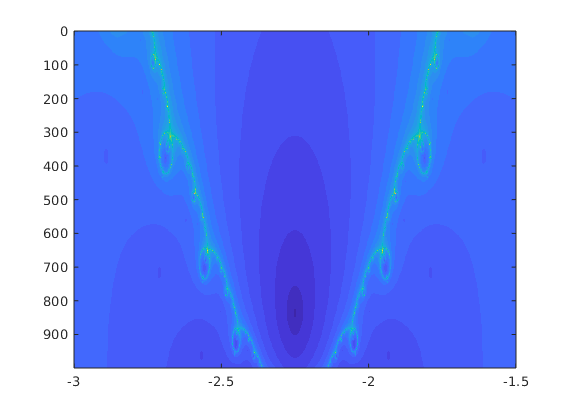
\includegraphics[keepaspectratio=true,scale=0.8]{map2.png}
\end{center}\end{figure}
\newpage

\subsection{Przykład 2}
Obszar działania metody: $[2,7]\times[3,11]$\newline
Wektor $a_k=[1,2,3,4,5,6]$\newline
Wizualizacja poszukiwania zer wielomianu:\newline

\begin{figure}[ht]
\begin{center}
\advance\leftskip-3cm
\advance\rightskip-3cm
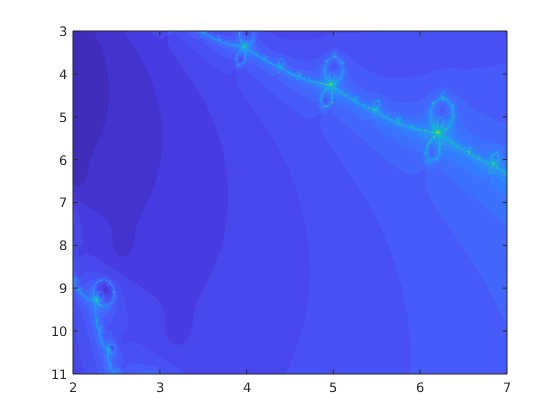
\includegraphics[keepaspectratio=true,scale=0.8]{map3.png}\newline
\end{center}\end{figure}
\newpage

\subsection{Przykład 3}
Obszar działania metody: $[-3,3]\times[3,3]$\newline
Wektor $a_k=[0,0,0,0,0,0,0,0,0,0,1]$\newline
Wizualizacja poszukiwania zer wielomianu:\newline

\begin{figure}[ht]
\begin{center}
\advance\leftskip-3cm
\advance\rightskip-3cm
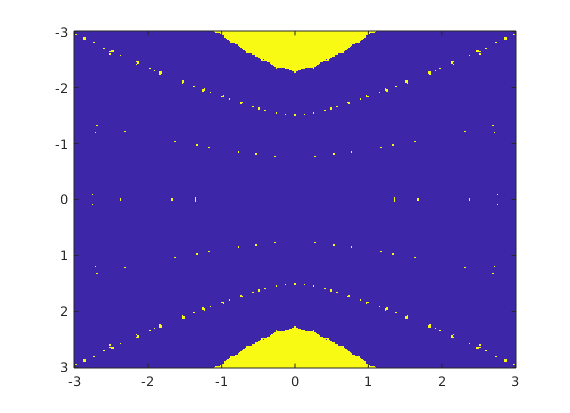
\includegraphics[keepaspectratio=true,scale=0.8]{map4.png}\newline
\end{center}\end{figure}
\newpage


\section{Menu}
\begin{figure}[ht]
\begin{center}
\advance\leftskip-3cm
\advance\rightskip-3cm
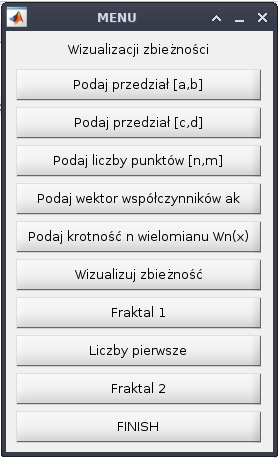
\includegraphics[keepaspectratio=true,scale=0.6]{menu1.png}

\end{center}\end{figure}
\newpage


\section{Kod rozwiązania} 
Funkcja obliczająca wartość i pochodne wielomianu rekurencyjnie:\newline
\lstinputlisting[style=Matlab-editor]{hermit.m}\newpage
Funkcja implementująca metodę Newtona:\newline 
\lstinputlisting[style=Matlab-editor]{newton.m}\newpage
Menu do obsługi powyższych funkcji: \newline
\lstinputlisting[style=Matlab-editor]{menu_wizualizacja.m}




\end{document}